\documentclass[../../../main.tex]{subfiles}
\begin{document}
On considère un ensemble fini $E$. Comme $E$ est fini, il est en bijection avec $\{0, \dots, n - 1\}$ où $n = |E|$. On cherche ici un moyen efficace de stocker et de manipuler une partition de $E$, c'est-à-dire une partition de $\{0, \dots, n-1\}$.

La manipulation de partitions de $E$ est équivalente à la manipulation de classes d'équivalence de $E$. Les classes d'équivalences apparaissent dans de nombreux problèmes dans lesquels les objets sont mis en relation, en particulier en théorie des graphes\footnote{Un graphe non valué est une relation sur un ensemble fini}.
\subsection{Principe et signature}
L'objectif est principalement de travailler sur les classes d'équivalences de la partition, c'est-à-dire :
\begin{itemize}
	\item construire les classes d'équivalence de la partition par unions itérés de classes
	\item lire la classe d'équivalence d'éléments quelconques
\end{itemize}
On en déduit la signature du type abstrait \textit{Partition} :

\textit{Partition} utilise \textit{Booléen}, \textit{Entier}
\begin{itemize}
	\item $creer(Entier:n)\rightarrow Partition$ renvoie une partition d'un ensemble à $n$ éléments en $n$ classes d'équivalences où chaque élément de l'ensemble est représentant de sa propre classe d'équivalence d'un seul élément.
	\item $unir(Partition, Entier:a, Entier:b)\rightarrow Partition$ renvoie la partition de $E$ où les classes d'équivalence de $\dot{a}$ et $\dot{b}$ sont unies en une seule classe d'équivalence
	\item $trouver(Partition, Entier:i)\rightarrow Entier$ renvoie $\dot{i}$ le représentant de la classe d'équivalence de $i$
\end{itemize}
Observe que pour chaque classe d'équivalence, on peut choisir, arbitrairement, un représentant. Par exemple, dans $\dfrac{\mathbb{Z}}{n\mathbb{Z}}$, $2\equiv 5\text{ mod }3$ et en considérant comme représentant de la classe le plus petit entier positif appartenant à la classe, on a $\dot{5} = \dot{2} = 2$.

La notation qui suit servira à visualiser le fonctionnement des deux fonctions $unir$ et $trouver$.

\textbf{Notation :} Prenons un ensemble $E = \{0, \dots, n-1\}$ qu'on partitionne en $k$ sous-ensembles disjoints $E_0, \dots, E_{k-1}$. Chaque $E_i$ a un représentant \textit{arbitraire} $r_i\in \{0, \dots, n-1\}$. On note alors $E_i = \{\dots\}_{r_i}$.\newline
On note finalement une partition de $E$ :
$$P = \{E_0, \dots, E_{k-1}\}$$
C'est-à-dire que :
$$E = \displaystyle\bigsqcup_{E\in P}E = \displaystyle\bigsqcup_{i=0}^{k-1} E_i$$

\textbf{Exemple :} Prenons l'ensemble $E = \{0, 1, 2, 3, 4, 5\}$. Sa partition la plus fine est constituée des $6$ classes $\{0\}_0, \dots, \{5\}_5$.
\begin{itemize}
	\item Initialement $P = \{\{0\}_0, \{1\}_1, \{2\}_2, \{3\}_3, \{4\}_4, \{5\}_5\}$
	\item $P\leftarrow unir(P, 0, 4) = \{\{0, 4\}_4, \{1\}_1, \{2\}_2, \{3\}_3, \{5\}_5\}$
	\item $P\leftarrow unir(P, 5, 1) = \{\{0, 4\}_4, \{1, 5\}_1, \{2\}_2, \{3\}_3\}$
	\item $trouver(P, 5) \rightarrow 1$
	\item $P \leftarrow unir(P, 5, 4) = unir(P, 1, 4) = \{\{0, 4, 1, 5\}_4, \{2\}_2, \{3\}_3\}$
	\item $trouver(P, 1) \rightarrow 4$
\end{itemize}
\subsection{Implantation}
On veut associer à chaque élément de $\{0, \dots, n-1\}$ le représentant de sa classe d'équivalence. C'est une fonction de $\{0, \dots, n-1\}$ dans $\{0, \dots, n-1\}$. Un tableau d'entiers convient très bien. Il suffit de lire le tableau pour trouver le représentant :
\begin{minted}[linenos=false]{c}
struct UnionFind {
	unsigned int *repr;
	unsigned int cardinal;
};

struct UnionFind unionfind_create(unsigned int cardinal) {
	struct UnionFind uf;
	uf.repr = (unsigned int*)malloc(cardinal * sizeof(unsigned int));
	uf.cardinal = cardinal;
	for (unsigned int i = 0; i < cardinal; i++) {
		uf.repr[i] = i;
	}
	return uf;
}

unsigned int unionfind_find(struct UnionFind uf, unsigned int e) {
	return uf.repr[e]; // logique... mais faux
}

void unionfind_union(struct UnionFind uf, unsigned a, unsigned b) {
	unsigned int r_a = unionfind_find(a);
	unsigned int r_b = unionfind_find(b);

	uf.repr[r_a] = r_b; // pourquoi pas... le choix est arbitraire
}
\end{minted}
\textbf{Remarque 1 :} le type \textit{Partition} est communément appelé \textit{UnionFind} de par le nom des deux opérations élémentaires fondamentales du type.

\textbf{Remarque 2 :} le code ci-dessus est dysfonctionnel au niveau du $unionfind\_find$. En effet, après l'union \mintinline{c}{uf.repr[r_a] = r_b;}, les éléments de représentant \mintinline{c}{r_a} ne sont plus trouvés correctement. Leur représentant est toujours \mintinline{c}{r_a} alors qu'il devrait être \mintinline{c}{r_b}. Il faudrait itérer une fois de plus. Une nouvelle union pourrait exiger d'itérer deux fois. En fait, tant qu'on a pas \mintinline{c}{uf.repr[r] = r}, on a pas encore trouvé le véritable représentant de la classe.

On corrige donc par : 
\begin{minted}[linenos=false]{c}
unsigned int unionfind_find(struct UnionFind uf, unsigned int e) {
	do {
		e = uf.repr[e];
	} while (e != uf.repr[e]); // tant que 'e' n'est pas le vrai représentant
	return e;
}
\end{minted}
Dans le pire des cas, il faut itérer sur toute la classe d'équivalence qui peut au maximum contenir tout l'ensemble, c'est-à-dire $n$ éléments. La complexité temporelle dans le pire cas est donc une fonction de $O(n)$.

\textbf{Reprise de l'exemple précédent :} on reprend l'ensemble $E = \{0, 1, 2, 3, 4, 5\}$ de l'exemple précédent. Le tableau des représentants est au départ :
$$T = [0, 1, 2, 3, 4, 5]$$
\begin{itemize}
	\item Après $unir(P, 0, 4)$, on a $T = [4, 1, 2, 3, 4, 5]$
	\item Après $unir(P, 5, 1)$, on a $T = [4, 1, 2, 3, 4, 1]$
	\item On a $trouver(P, 5) = 1$ car $T[5] = 1$ puis $T[1] = 1$, donc $1$ est le vrai représentant de $5$
	\item Après $unir(P, 5, 4) = unir(P, 1, 4)$, on a $T = [4, 4, 2, 3, 4, 1]$
	\item On a $trouver(P, 5) = 4$ car $T[5] = 1$ puis $T[1] = 4$ puis $T[4] = 4$ donc $4$ est le vrai représentant de $5$
\end{itemize}
\subsection{Amélioration de la complexité dans le pire cas}
Les successeurs d'un représentant de classe dans le tableau forment une arborescence : 
\begin{center}
	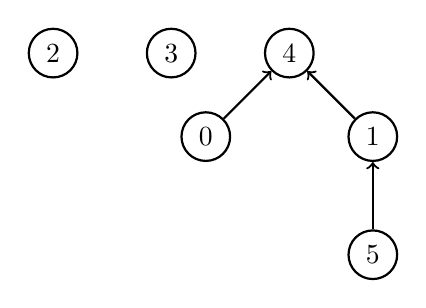
\begin{tikzpicture}[node distance={15mm}, thick, main/.style = {draw, circle}] 
		% Sommets :
		\node[main] (2) {$2$};
		\node[main] (3) [right of=2] {$3$};
		\node[main] (4) [right of=3] {$4$};
		\node[main] (0) [below left of=4] {$0$}; 
		\node[main] (1) [below right of=4] {$1$};
		\node[main] (5) [below of=1] {$5$};
		% Arêtes
		\draw[<-] (4) -- (0);
		\draw[<-] (4) -- (1);
		\draw[<-] (1) -- (5);
	\end{tikzpicture}
	\captionof{figure}{Forêt représentative de la partition $P$ de l'exemple\label{fig:foret_partition}}
\end{center}
Si on doit parcourir toute la classe d'équivalence pour trouver le représentant, c'est que les successeurs de l'élément dont on cherche le représentant forment tout l'arbre. C'est donc une liste. L'objectif est d'éviter ce cas de figure. Si on parvient à éviter les arborescences ``filiformes'', on améliore considérablement le temps de parcours.

Dans le meilleur des cas, pour tout élément $e\in E$, on obtient le représentant de $e$ directement par \mintinline{c}{uf.repr[e]}.
\subsubsection{Union pondéré}
Prenons la partition représentée par la figure \ref{fig:foret_partition}. Supposons qu'on veuille effectuer $unir(P, 3, 4)$. On a deux possibilités :

\begin{minipage}{0.5\textwidth}
\begin{center}
	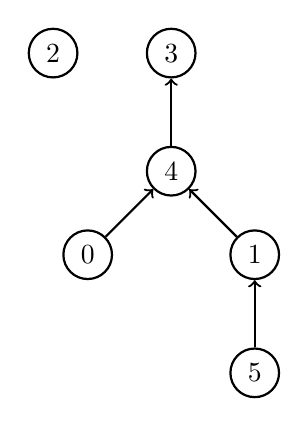
\begin{tikzpicture}[node distance={15mm}, thick, main/.style = {draw, circle}] 
		% Sommets :
		\node[main] (2) {$2$};
		\node[main] (3) [right of=2] {$3$};
		\node[main] (4) [below of=3] {$4$};
		\node[main] (0) [below left of=4] {$0$}; 
		\node[main] (1) [below right of=4] {$1$};
		\node[main] (5) [below of=1] {$5$};
		% Arêtes
		\draw[<-] (3) -- (4);
		\draw[<-] (4) -- (0);
		\draw[<-] (4) -- (1);
		\draw[<-] (1) -- (5);
	\end{tikzpicture}
\end{center}
\end{minipage}
\begin{minipage}{0.5\textwidth}
\begin{center}
	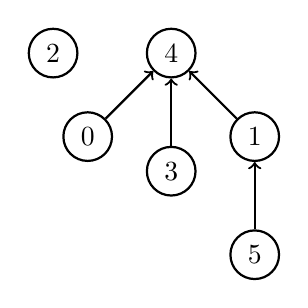
\begin{tikzpicture}[node distance={15mm}, thick, main/.style = {draw, circle}] 
		% Sommets :
		\node[main] (2) {$2$};
		\node[main] (4) [right of=2] {$4$};
		\node[main] (3) [below of=4] {$3$};
		\node[main] (0) [below left of=4] {$0$}; 
		\node[main] (1) [below right of=4] {$1$};
		\node[main] (5) [below of=1] {$5$};
		% Arêtes
		\draw[<-] (4) -- (3);
		\draw[<-] (4) -- (0);
		\draw[<-] (4) -- (1);
		\draw[<-] (1) -- (5);
	\end{tikzpicture}
\end{center}
\end{minipage}

\begin{minipage}{0.5\textwidth}
\centering \captionof{figure}{Choix de $3$ comme représentant}\label{fig:choix_union_3}
\end{minipage}
\begin{minipage}{0.5\textwidth}
\centering \captionof{figure}{Choix de $4$ comme représentant}\label{fig:choix_union_4}
\end{minipage}

Le second choix est évidemment optimal. Le critère est de choisir comme enfant l'arbre le moins haut. On ajoute donc dans \mintinline{c}{struct UnionFind} un tableau \textsf{highs}, rempli de $0$ à la création et on modifie la routine d'union par :
\begin{minted}[linenos=false]{c}
#define MAX(X, Y) (((X) < (Y)) ? (Y) : (X))

void unionfind_union(struct UnionFind uf, unsigned a, unsigned b) {
	unsigned int r_a = unionfind_find(a);
	unsigned int r_b = unionfind_find(b);
	if (uf.highs[r_a] > uf.highs[r_b]) {
		uf.repr[r_b] = r_a;
	} else {
		uf.repr[r_a] = r_b;
		uf.highs[r_b] = MAX(1 + uf.highs[r_a], uf.highs[r_b]);
	}
}
\end{minted}
\textbf{Notation :} Après $i$ opérations d'unions sur la partition, on note pour tous $x\in E$ :
\begin{itemize}
	\item $t_i(x)$ le nombre d'éléments de l'arbre de racine $x$ après $i$ unions sur la partition
	\item $h_i(x)$ la hauteur de l'arbre de racine $x$ après $i$ unions sur la partition
\end{itemize}
On observe que $t_0(x) = 1$ et $h_0(x) = 0$.

$h_i(x)$ correspond à \mintinline{c}{uf.highs[x]} après $i$ opérations d'union sur la partition.

\proposition{Borne sur la hauteur} pour tout $x\in E$, pour tout $i\in \mathbb{N}$, $t_i(x)\geq 2^{h_i(x)}$.

Il s'ensuit que pour $n = Card(E)$, on a $log_2(n) \geq log_2(t_i(x))\geq h_i(x)$. La complexité temporelle dans le pire cas de $trouver$ est donc en $O(log_2(n))$.

\textbf{Démonstration :} On pose pour tout $k\in\mathbb{N}$ la proposition $P_k : \forall x\in E, t_k(x)\geq 2^{h_k(x)}$.

\underline{Initialisation :} pour $k = 0$, $t_0(x) = 2^{h_0(x)}$ car $t_0(x) = 1$ et $h_0(x) = 0$

\underline{Hérédité :} Soit $k\in\mathbb{N}$. Soient $x, y\in E$. Supposons $P_k$.

On calcul $union(P, x, y)$ :
\begin{itemize}
	\item Si $h_i(x) > h_i(y)$, alors $h_{i+1}(x) = h_i(x)$ et $t_{i+1}(x) = t_i(x) + t_i(y) \geq t_i(x) \geq 2^{h_{i}(x)} = 2^{h_{i+1}(x)}$. La hauteur et le nombre d'éléments de $y$ sont inchangés. OK.
	\item Si $h_i(x) \leq h_i(y)$, on a déjà $t_{i+1}(y) = t_i(y) + t_i(x)$. Ensuite $h_{i+1}(y) = max(h_i(y), 1 + h_i(x))$. Si $h_{i+1}(y) = h_i(y)$, tout est OK. Sinon, par l'inégalité supposée et puisque les hauteurs sont entières, on a $h_{i+1}(y) = 1 + h_i(x) = 1 + h_i(y)$. D'où $t_{i+1}(y) \geq 2^{h_i(y) + 1}\geq 2^{h_{i+1}(y)}$ . OK
\end{itemize}

\underline{Conclusion :} $(P_k)_{k\in\mathbb{N}}$ est initialisée et héréditaire, donc pour tout $k\in\mathbb{N}$, $P_k$ est vraie.
\subsubsection{Compression des chemins}
La fonction $unir$ est optimisée. On s'intéresse maintenant à optimiser $trouver$. 

Lorsqu'on parcours l'arbre pour trouver le représentant d'un élément, on peut au passage modifier cet arbre pour que tous les sommets visités par ce parcours soient ``recollés'' directement au représentant. En C, cela donne :
\begin{minted}[linenos=false]{c}
unsigned int unionfind_find(struct UnionFind uf, unsigned int e) {
// Calcul du représentant
	unsigned r = e;
	do {
		r = uf.repr[r];
	} while (r != uf.repr[r]); // tant que 'r' n'est pas le vrai représentant
// Compression du chemin : on parcours à nouveau le chemin pour lier directement au vrai représentant 'r'
	do {
		unsigned tmp = e;
		e = uf.repr[e];
		uf.repr[tmp] = r; // le sommet est lié directement au représentant
	} while (e != uf.repr[e])
	return r;
}
\end{minted}
La première fois qu'on cherche le représentant de $e$, on double le nombre d'opérations effectués, pour effectuer la compression. Cependant, toutes les prochaines opérations $trouver$ sur les éléments du chemin seront beaucoup plus rapide. C'est donc une optimisation au niveau global.
\subsection{Exercices}

\end{document}